\chapter{Implementation}\label{chapter:Implementation}

\section{Project Structure}

The Python bindings for the sys\_sage library are encapsulated within a dedicated wrapper file. This file serves as the primary interface between the C++ library and the Python environment, ensuring a structured and maintainable codebase. The general layout of this file is as follows:
\begin{figure}[htpb]
    \centering
    \begin{tabular}{c}
        \begin{lstlisting}[language=C++]
            #include <pybind11/pybind11.h>
            #include <pybind11/stl.h>
            #include <pybind11/attr.h>
            #include "sys-sage.hpp"
            
            // Global variables and helper functions
            
            PYBIND11_MODULE(sys_sage, m) {
                // Expose C++ Macros to Python
                m.attr("COMPONENT_NONE") = SYS_SAGE_COMPONENT_NONE;
            
                // Bind the Component class
                py::class_<...>(m, "Component", ..., "Generic Component")
                    // Bind the constructor(s)
                    .def(py::init<...>())
                    // Bind member functions
                    .def("InsertChild", &Component::InsertChild, ...)
                    // Bind properties (getters and setters)
                    .def_property("parent", &Component::GetParent, &Component::SetParent, ...);
            
                // Bind module-level functions
                m.def("parseCccbenchOutput", &parseCccbenchOutput, ...);
            }
            \end{lstlisting}
    \end{tabular}
    \caption[Structure of the wrapper file]{The structure of the wrapper file.}\label{fig:wrapper-structure}
  \end{figure}


This structure is designed to provide a clear and organized layout, facilitating easy navigation and modification of the bindings. The file is segmented into distinct sections, each serving a specific purpose:

\begin{itemize}
    \item   \textbf{Include Directives:} Essential header files, including those from pybind11 and the sys\_sage library, are included to provide the necessary functionalities.
    \item   \textbf{Global Variables and Helper Functions:} This section accommodates any global variables or helper functions required for the bindings.
    \item   \textbf{PYBIND11\_MODULE Macro:} This macro defines the Python module and its contents. Within this macro, the following elements are defined:
        \begin{itemize}
            %TODO This is not really true
            \item   \textbf{DATA:} C++ macros are exposed to Python in form of module attributes, allowing Python code to use these as constants.
            \item   \textbf{Class Bindings:} C++ classes are bound to Python classes using \verb|py::class_<>|. This includes defining constructors, methods, and properties.
            \item   \textbf{Module Functions:} C++ functions that are not class methods are bound to the Python module itself.
        \end{itemize}
\end{itemize}

This structured approach ensures that the bindings are well-organized and easy to maintain, providing a solid foundation for the Python interface of the sys\_sage library.


\section{Object-Oriented Programming with pybind11}

\subsection{Class Definitions}

Python and C++ both offer object-oriented programming. C++ differentiates between structs and classes, while Python primarily uses classes. pybind11 allows C++ structs as well as classes to be bound to act like Python classes.

For each functionality, a table is provided for comparison.
        
\begin{table}[htbp]
\centering
\begin{tabular}{|l|l|}
\hline
\textbf{C++ implementation} &
\begin{lstlisting}[language=C++]
class Component {
    // ...
};
\end{lstlisting}
\\ \hline
\textbf{Pybind11-Binding} &
\begin{lstlisting}[language=C++]
py::class_<Component, std::unique_ptr<Component, py::nodelete>>(
    m, "Component", "Generic Component"
);
\end{lstlisting}
\\ \hline
\textbf{C++ usage} &
\verb|Component;| \\ \hline
\textbf{Python usage} &
\verb|sys_sage.Component| \\ \hline
\end{tabular}
\caption{Class Definition Comparison}
\label{tab:class_definition}
\end{table}

Header files define classes. pybind bindings are defined in the binding file within the module. To use \verb|sys-sage| in C++, we need to include \verb|syssage.hpp| in the project. To use \verb|sys-sage| in Python, we need to include \verb|sys_sage|, where we can also rename the module.

We can see that pybind bindings are straightforward. We use \verb|py::class_<T>| where \verb|T| is the template input, in this case, \verb|Component|. As mentioned in the previous chapter, for pybind to indicate that component objects should not be destroyed by Python, we use \verb|std::unique_ptr<T>| as holder type for the Component class, and we add a delete function, that is \verb|py::nodelete|. There are also other methods to define how Python should handle the underlying C++ objects.

The \verb|py::class_| takes the module, class name , and class documentation as arguments.

%*TODO:* Improve Documentation. Helpful feature to add documentation to the project and help users understand usage better.

\subsection{Constructor}

If we would define a class in native Python, it might look like this:

\begin{lstlisting}[language=Python, xleftmargin=4em, frame = single]
class Example(self):
    def __init__(self, id, name):
        self.id = id
        self.name = name
\end{lstlisting}

With pybind, we can take already defined Constructors of C++ implementation and can use the convenience function \verb|init<>()| that binds automatically the C++ Constructors.

\begin{table}[htbp]
\centering
\begin{tabular}{|l|l|}
\hline
\textbf{C++ implementation} &
\begin{lstlisting}[language=C++]
Component(
    int id = 0,
    string name = "unknown",
    int componentType = SYS_SAGE_COMPONENT_NONE
);
\end{lstlisting}
\\ \hline
\textbf{Pybind11-Binding} &
\begin{lstlisting}[language=C++]
.def(
    py::init<int, string, int>(),
    py::arg("id") = 0,
    py::arg("name") = "unknown",
    py::arg("type") = SYS_SAGE_COMPONENT_NONE
)
\end{lstlisting}
\\ \hline
\textbf{C++ usage} &
\verb|new Component();| \\ \hline
\textbf{Python usage} &
\verb|sys_sage.Component()| \\ \hline
\end{tabular}
\caption{Constructor Comparison}
\label{tab:constructor}
\end{table}

C++ implementation provides a bunch of Constructors for Component-Class and Subclasses. In our use case, Pybind's convenience function is indeed convenient.

For all functions and properties we want to bind to, we use \verb|.def(...)|. That also applies to initialization function, where we use the function \verb|py::init<T>()|. As one can see, this is a template function, and we replace \verb|T| with all the types of the Arguments there are defined in the C++ Constructor. In our example case, we have \verb|int|, \verb|string|, \verb|int| in this order.

As in every definition of a function in the bindings, we can use \verb|py::arg| to not only define default values but also we can give the argument names for the documentation. In this case, this might look like this: \verb|py::arg("id") = 0|. Instead of this, there is also a shorthand notation that would look like this: \verb|"id"_a=0|. However, the literal operator must be made visible before with \verb|using namespace pybind11::literals|.
\begin{lstlisting}[language=C++, xleftmargin=4em, frame = single]
            // Component-constructor without parent
            .def(
                py::init<int, string, int>(),
                py::arg("id") = 0,
                py::arg("name") = "unknown",
                py::arg("type") = SYS_SAGE_COMPONENT_NONE
            )
            
            // Component-constructor with parent
            .def(
                py::init<Component *, int, string, int>(),
                py::arg("parent"),
                py::arg("id") = 0,
                py::arg("name") = "unknown",
                py::arg("type") = SYS_SAGE_COMPONENT_NONE
            )
\end{lstlisting}
% *TODO:* Add shorthand notation in pybinds.
\subsection{Inheritance}

If we had to define Inheritance in Python, we can do it like this:
\newpage
\begin{lstlisting}[language=Python, xleftmargin=4em, frame = single]
class Vehicle:
    def honk(self):
        print("Honk!")

class Car(Vehicle):
    def drive(self):
        print("Vroom!")

my_car = Car()
my_car.honk()
my_car.drive()
\end{lstlisting}

The \verb|sys_sage| library has \verb|Component| as a generic class and many Component-Types as Subclasses. Inheritance should work properly, and indeed Pybind supports that.

\begin{table}[htbp]
\centering
\begin{tabular}{|l|l|}
\hline
\textbf{C++ implementation} &
\begin{lstlisting}[language=C++]
class Topology : public Component {
    // ...
};
\end{lstlisting}
\\ \hline
\textbf{Pybind11-Binding} &
\begin{lstlisting}[language=C++]
py::class_<
    Topology,
    std::unique_ptr<Topology, py::nodelete>,
    Component
>(m, "Topology")
\end{lstlisting}
\\ \hline
\textbf{C++ usage e.g.} &
\begin{lstlisting}[language=C++]
t.GetId();  // t is Topology, but can access Component's 
            // attributes and functions
\end{lstlisting}
\\ \hline
\textbf{Python usage} &
\verb|t.id # Works as in C++| \\ \hline
\end{tabular}
\caption{Inheritance Comparison}
\label{tab:inheritance}
\end{table}

The super-class is given as input in the template of \verb|py::class_<>|. Pybind will automatically care that all the functions and attributes from the super class are accessible to the Subclass. Multiple inheritance is also allowed. This is not yet needed but maybe in the future.

\subsection{Functions}

With pybind, binding functions is quite simple. Consider this C++ function for example:

\begin{table}[htbp]
\centering
\begin{tabular}{|l|l|}
\hline
\textbf{C++ implementation} &
\begin{lstlisting}[language=C++]
void Component::InsertChild(Component * child){
    // ...
}
\end{lstlisting}
\\ \hline
\textbf{Pybind11-Binding} &
\begin{lstlisting}[language=C++]
.def(
    "InsertChild",
    &Component::InsertChild,
    py::arg("child")
)
\end{lstlisting}
\\ \hline
\textbf{C++ usage e.g.} &
\verb|c->InsertChild(child);| \\ \hline
\textbf{Python usage} &
\verb|c.InsertChild(child)| \\ \hline
\end{tabular}
\caption{Function Comparison}
\label{tab:function}
\end{table}

In \verb|.def()|, the first argument is the name of the method. Normally in Python, the convention is to use snake-case for the method-name. In this case, we use the same name as in the C++ implementation. For some other specific methods, we use more simple names, but more on this in the “Attribute”-Section. The next argument is the C++ function to bind, and the last argument is the argument name for the function. This is not necessary, but it helps for documentation and allows usage of keyword arguments.

\subsection{Overloaded methods}

To use overloaded methods, we need to pick up the method signature to map the correct overloaded method.
\newpage
\begin{table}[htbp]
\centering
\begin{tabular}{|l|l|}
\hline
\textbf{C++ implementation} &
\begin{lstlisting}[language=C++]
void Component::PrintSubtree() {
    PrintSubtree(0);
}

void Component::PrintSubtree(int level) {
    PrintSubtree(0);
}
\end{lstlisting}
\\ \hline
\textbf{Pybind11-Binding} &
\begin{lstlisting}[language=C++]
.def(
    "PrintSubtree",
    (void (Component::)()) &Component::PrintSubtree,
    "Print the subtree of the component"
)

.def(
    "PrintSubtree",
    (void (Component::)(int)) &Component::PrintSubtree,
    "Print the subtree ..."
)
\end{lstlisting}
\\ \hline
\textbf{C++ usage e.g.} &
\begin{lstlisting}[language=C++]
c.PrintSubtree();
c.PrintSubtree(0);
\end{lstlisting}
\\ \hline
\textbf{Python usage} &
\begin{lstlisting}[language=Python]
c.PrintSubtree()
c.PrintSubtree(0)
\end{lstlisting}
\\ \hline
\end{tabular}
\caption{Overloaded Methods Comparison}
\label{tab:overloaded_methods}
\end{table}

The only difference to “normal” binding is that with overloading, we add the method signature, which is in this case \verb|void (Component::) ()| and \verb|void (Component::) (int)| respectively, which we add before \verb|&Component::PrintSubtree|.

%*TODO:* Maybe add more?

\subsection{Lambda functions}

In some cases, we don't have any C++ function we can bind to. This is because either we want to add some additional methods or there is some logic needed before the C++ function can be called.

For the first case, we have this example:
\newpage
\begin{lstlisting}[language=C++, xleftmargin=4em, frame = single]
.def(
    "__bool__",
    [](Component\& self){
        std::vector<Component*> children = self.GetChildren();
        return !children->empty();
    }
)
\end{lstlisting}

Here, we define the bool-function, which is called whenever we want to extract a bool value from an object of any type, in this case Component-type. Within the lambda function, we check if the Component object has any children. This is convenient because we can then in Python do this:

\begin{lstlisting}[language=Python,xleftmargin=4em, frame = single]
comp = sys_sage.Component()
# ...
if comp:
    # comp has children
else:
    # comp has no children
\end{lstlisting}

So this is an example for an extra feature that is not there in the base implementation of \verb|sys_sage| in C++. But this also shows that there it is quite straightforward to add more functionalities with a few lines of code.

\subsection{Module functions}

Previously presented methods are class methods, but there are also module functions that are not to be accessed over an object but see for yourself:

\begin{table}[htbp]
\centering
\begin{tabular}{|l|l|}
\hline
\textbf{C++ implementation} &
\begin{lstlisting}[language=C++]
int parseCapsNumaBenchmark(
    Component* rootComponent,
    string benchmarkPath,
    string delim
){
    // ...
}
\end{lstlisting}
\\ \hline
\textbf{Pybind11-Binding} &
\begin{lstlisting}[language=C++]
m.def(
    "parseCapsNumaBenchmark",
    \&parseCapsNumaBenchmark,
    py::arg("root"),
    py::arg("benchmarkPath"),
    py::arg("delim") = ";"
);
\end{lstlisting}
\\ \hline
\textbf{C++ usage e.g.} &
\verb|parseCapsNumaBenchmark( root, “benchmark.csv”, “;”);| \\ \hline
\textbf{Python usage} &
\verb|sys_sage.parseCapsNumaBenchmark(root, "benchmark.csv", ";")| \\ \hline
\end{tabular}
\caption{Module Function Comparison}
\label{tab:module_functions}
\end{table}

So this is quite similar to the class methods, but here we assign the function to the module interface object \verb|m|.
\newpage


\section{Attributes}

This section delves into the intricacies of attributes within the \verb|sys_sage| library, expanding on the object-oriented programming concepts discussed earlier. Attributes warrant a dedicated discussion due to the numerous special cases and module-specific considerations.

\subsection{Module Attributes}

\verb|sys_sage| employs macros in its C++ implementation to define component and datapath types. To maintain consistency and offer similar functionality in Python, we utilize module attributes. 

\begin{table}[htbp]
\centering
\begin{tabular}{|l|l|}
\hline
\textbf{C++ implementation} & \begin{lstlisting}[language=C++]
#define SYS_SAGE_COMPONENT_NONE 1 
\end{lstlisting} \\ \hline
\textbf{Pybind11-Binding} & \begin{lstlisting}[language=C++]
m.attr("COMPONENT_NONE") = SYS_SAGE_COMPONENT_NONE;
\end{lstlisting} \\ \hline
\textbf{C++ usage e.g.} & \verb|c.CountAllSubcomponentsByType(SYS_SAGE_COMPONENT_NONE);| \\ \hline
\textbf{Python usage} & \verb|c.CountAllSubcomponentsByType(sys_sage.COMPONENT_NONE)| \\ \hline
\end{tabular}
\caption{Module Attribute Comparison}
\label{tab:module_attributes}
\end{table}

In C++, these macros are preprocessed and replaced with their corresponding integer values. In Python, they are treated as exported variables, registered using the \verb|attr| function, effectively making them module attributes. Pybind handles the necessary type casting, as all macros resolve to integers.

A naming convention is employed where the “SYS\_SAGE” prefix is omitted from the Python attribute names to avoid redundancy. As demonstrated in the example, the attributes are accessed via \verb|sys_sage.COMPONENT_NONE|.
%TODO Add acronym
A significant advantage of the Python implementation is its enhanced documentation capabilities. A user's \ac{IDE} or the \verb|help(sys_sage)| function in python can display all module attributes within the DATA section, aiding users in selecting the appropriate options.

\subsection{Properties (Default Attributes)}

In C++, class attributes are typically private and accessed through setter and getter methods. However, this pattern is not idiomatic in Python. Pybind offers the \verb|def_property| function to bind setter and getter methods to Python properties, providing a more natural syntax.

\begin{table}[htbp]
\centering
\begin{tabular}{|l|l|}
\hline
\textbf{C++ implementation} & \begin{lstlisting}[language=C++]
class Component{
  private:
     string name;
};
...
void SetName(string name){...}
string GetName(){...}
\end{lstlisting} \\ \hline
\textbf{Pybind11-Binding} & \begin{lstlisting}[language=C++]
.def_property("name", &Component::GetName, &Component::SetName)
\end{lstlisting} \\ \hline
\textbf{C++ usage e.g.} & \begin{lstlisting}[language=C++]
string name = c.GetName();
c.SetName("name");
\end{lstlisting} \\ \hline
\textbf{Python usage} & \begin{lstlisting}[language=Python]
name = c.name
c.name = "name"
\end{lstlisting} \\ \hline
\end{tabular}
\caption{Property Comparison}
\label{tab:properties}
\end{table}
\newpage
This syntax is more intuitive for Python users. Pybind also provides \verb|def_property_readonly| for read-only properties, such as the \verb|id| attribute.

\begin{table}[htbp]
\centering
\begin{tabular}{|l|l|}
\hline
\textbf{C++ implementation} & \begin{lstlisting}[language=C++]
class Component{
  private:
     int id;
};
...
string GetId(){...}
\end{lstlisting} \\ \hline
\textbf{Pybind11-Binding} & \begin{lstlisting}[language=C++]
.def_property_readonly("id", &Component::GetId)
\end{lstlisting} \\ \hline
\textbf{C++ usage e.g.} & \verb|int id = c.GetId();| \\ \hline
\textbf{Python usage} & \verb|id = c.id| \\ \hline
\end{tabular}
\caption{Read-only Property Comparison}
\label{tab:readonly_properties}
\end{table}

\subsection{Dynamic Attributes}

Python natively supports dynamic attributes, allowing users to add attributes to objects at runtime.

\begin{lstlisting}[language=Python, xleftmargin=4em, frame = single]
class Dog():
    # no attributes defined here
    ...

d = Dog()
d.hungry = True
d.hungry # True
\end{lstlisting}

This behavior is desirable for \verb|sys_sage| components and datapaths, especially considering the C++ implementation's \verb|std::map<std::string, void*> attrib| which facilitates dynamic attribute storage.

\subsubsection{Attribute-Map}

The \verb|attrib| map offers high flexibility and performance by storing \verb|void*| pointers with string keys. This allows for storing both C++ types for the default attributes and Python types for custom attributes. Users should be able to modify these attributes, mirroring the C++ base implementation.

There are multiple possibilities to connect the \verb|attrib| map to Python attributes. For example, Pybind can activate Python's native dynamic attribute functionality using \verb|py::dynamic_attr()|.

\begin{lstlisting}[language=C++, xleftmargin=4em, frame = single]
py::class_<Component, std::unique_ptr<Component, py::nodelete>>(m, "Component", py::dynamic_attr(),"Generic Component");
\end{lstlisting}

This enables dynamic attribute usage in Python:

\begin{lstlisting}[language=Python, xleftmargin=4em, frame = single]
c = sys_sage.Component()
c.dynamic = "attribute"
c.dynamic # returns "attribute"
\end{lstlisting}

However, this approach conflicts with \verb|def_property()|. If we want to conntect the \verb|attrib| map to Python attributes we need to override the \verb|__setattr__| and \verb|__getattr__| methods, but this breaks property functionality. Handling properties like \verb|name| or \verb|id| in custom setter and getter methods, that we define would work as well, but results in bloated code. Therefore, an alternative solution is considered. This approach uses the \verb|[]| operator to access attributes, overriding \verb|__getitem__| and \verb|__setitem__|.

\begin{lstlisting}[language=Python, xleftmargin=4em, frame = single]
c = sys_sage.Component()
# solution with dynamic attributes
c.example = "test"      # calls __setattr__
c.example               # calls __getattr__
# solution with items
c["example"] = "test"   # calls __setitem__
c["example"]            # calls __getitem__
\end{lstlisting}

This solution avoids conflicts with other functions.

% The implementation in the bindings is as follows:

% \begin{lstlisting}[language=C++, xleftmargin=4em, frame = single]
% .def("__setitem__", [](Component& self, const std::string& name, py::object value) {
%     set_attribute(self,name, value);
% })
% .def("__getitem__", [](Component& self, const std::string& name) {return get_attribute(self,name);
% })
% .def("__getitem__", [](Component& self, int pos) {
%     return get_attribute(self,pos);
% })
% .def("__delitem__", [](Component& self, const std::string& name) {remove_attribute(self,name);
% })
% \end{lstlisting}

Overloaded \verb|__getitem__| methods allow access by key and index. The following example demonstrates this:

\begin{lstlisting}[language=Python, xleftmargin=4em, frame = single]
c["example"] = "test"
c[0]  # returns "test" if "example" is the only custom attribute
\end{lstlisting}
In the Python implementation, accessing and modifying attributes is designed to be user-friendly. The getter and setter methods for attributes are implemented to handle Python objects of any type or default attributes. This abstraction allows users to interact with custom attributes without explicit type casting. For default attributes, users need to be aware of the corresponding Python types.

In contrast, the C++ implementation requires more explicit memory management and type handling for attribute manipulation. The following code snippet illustrates the process of updating and retrieving an attribute in C++:

\begin{lstlisting}[language=C++, xleftmargin=4em, frame = single]
// Update Attribute
std::string key = "example";
if (c->attrib.find(key) != c->attrib.end()) {
    std::string* oldValue = static_cast<std::string*>(c->attrib[key]);
    delete oldValue; // Free the old value
}
std::string* newValue = new std::string("test"); // Allocate new value
c->attrib[key] = static_cast<void*>(newValue); // Update the map

// Retrieve Attribute
if (c->attrib.find(key) != c->attrib.end()) {
    std::string* retrievedValue = static_cast<std::string*>(c->attrib[key]);
    std::cout << "Value: " << *retrievedValue << std::endl;
} else {
    std::cout << "Key not found." << std::endl;
}
\end{lstlisting}

As demonstrated in the code, updating an attribute in C++ involves checking for the existence of the key, explicitly freeing the memory associated with the old value, allocating memory for the new value, and then updating the attribute map with a void pointer. Similarly, retrieving an attribute requires casting the void pointer back to the expected type after verifying the key's existence. This manual memory management and type casting in C++ contrasts with the more dynamic and implicit handling of attributes in the Python interface provided by Pybind11.
In the following we briefly explain the helper functions that are used:

The \verb|set_attribute| function examines default values, converts data to C++ types, encapsulates Python data types in shared pointers, and stores them in the \verb|attrib_map|. The \verb|get_attribute| function retrieves attributes using a key or an index and casts the \verb|void*| pointers to their appropriate types. The \verb|del_attribute| function removes attributes from the map.

For the Component class the second approach, using items, was chosen for its simplicity and compatibility with existing properties. For Datapaths however dynamic attributes were enabled. Since the \verb|attrib| map is not being used in the xml export and import functionality we use the native Python dynamic attributes there.

\section{XML Export}

\subsection{Original Implemented Functionality}

The base C++ implementation of \verb|sys_sage| includes XML export functionality, which traverses the topology and generates an XML representation of it. XML's hierarchical structure is well-suited for representing topologies, where the topology itself is the root node, cores and threads are leaf nodes, and various components reside in between.

XML properties are utilized to represent default attributes such as \verb|id|, \verb|name|, \verb|type|, and type-bound memory attributes like \verb|size|. Datapaths are also included, with attributes like \verb|src|, \verb|target|, \verb|orientation|, \verb|latency|, and \verb|bandwidth|.

Dynamic attributes, which users can add in C++, are represented as separate XML nodes:

\begin{lstlisting}[language=xml, xleftmargin=4em, frame = single]
<Attribute name="GPU_Clock_Rate">
    <GPU_Clock_Rate frequency="2.000000" unit="MHz"/>
</Attribute>
\end{lstlisting}

Since the \verb|attrib| map in C++ stores attributes as \verb|void*|, the XML export function requires user-defined functions to parse custom attribute types. Users can define up to two functions:

\begin{lstlisting}[language=C++, xleftmargin=4em, frame = single]
std::function<int(string,void*,string*)> search_custom_attrib_key_fcn;
std::function<int(string,void*,xmlNodePtr)> search_custom_complex_attrib_key_fcn;
\end{lstlisting}

The first function returns a string representation of the attribute, while the second allows for creating more complex XML nodes. The export function can be called as follows:

\begin{lstlisting}[language=C++, xleftmargin=4em, frame = single]
exportToXml(
    root, 
    path, 
    search_custom_attrib_key_fcn, 
    search_custom_complex_attrib_key_fcn
);
\end{lstlisting}

\subsection{Process Description}

The Python implementation of \verb|exportToXml| mirrors the C++ functionality, allowing users to define custom parsing functions as in this example:

\begin{lstlisting}[language=Python, xleftmargin=4em, frame = single]
def search_custom(key: str, value) -> str:
    if "example" in key:
        return str(value)+"test"
    return None

def search_custom_complex(key: str, value) -> str:
    return "<root><Attribute key=\"" + str(key) + "\" value=\"" + str(value) + "\"/><root>"
\end{lstlisting}

The \verb|key| is always a string, while \verb|value| can be any Python type. The return value must be a string, representing either a simple value or an XML node respectively. When creating the XML node string for complex attributes the target XML information is incapsulated in a tag that is ommitted in the parsing operation. XML parsing modules like \verb|xml.etree.ElementTree|\cite{xml-etree} can be used to construct complex XML nodes.

The Python export function can be called as follows:

\begin{lstlisting}[language=Python, xleftmargin=4em, frame = single]
sys_sage.exportToXml(root, "out.xml", search_custom, search_custom_complex)
\end{lstlisting}

% The Pybind bindings are defined as follows:

% \begin{lstlisting}[language=C++, xleftmargin=4em, frame = single]
% m.def("exportToXml", [](Component& root, string xmlPath, std::optional<py::function> print_att = std::nullopt, std::optional<py::function> print_catt = std::nullopt) {
%         if(print_att)
%             print_attributes = *print_att;
%         if(print_catt)
%             print_complex_attributes = *print_catt;
%         exportToXml(&root, xmlPath,print_att ? xmldumper : nullptr,print_catt ? xmldumper_complex : nullptr);
%     },py::arg("root"), py::arg("xmlPath") = "out.xml", py::arg("print_att") = py::none(), py::arg("print_catt") = py::none());
% \end{lstlisting}

Global variables are used to store the user-defined functions. Two helper functions are used to translate between Python and C++ types. The helper functions implement the required functions with the correct signature for the XML-export function and within the helper functions the user-defined Python functions - previously stored in the global variables - are called to achieve the desired functionality. Default attributes are skipped, but this can be changed in the future.

\subsection{Helper Functions}

In the following we explain which steps are performed by the helper functions:

\subsubsection{Simple Attributes}
\begin{enumerate}
\item Check if the attribute is a default attribute. If yes, skip it.
\item Cast the \verb|void*| to a Python object.
\item Call the user-defined Python function, passing the key and value (Python object).
\item Cast the returned Python string to a C++ string.
\item Store the string in the return string pointer.
\end{enumerate}

\subsubsection{Complex Attributes}
\begin{enumerate}
\item Follow steps 1-3 for simple attributes.
\item Expect user-defined function to return XML node as a Python string.
\item Convert Python string to C++ string.
\item Parse the XML node using \verb|xmlParseDoc| \cite{libxml2-docu} and add it to the XML node.
\end{enumerate}

% \begin{lstlisting}[language=C++, xleftmargin=4em, frame = single]
% xmlDocPtr doc = xmlParseDoc((const xmlChar*)xml_str.c_str());
% xmlNodePtr root = xmlDocGetRootElement(doc);
% xmlAddChild(node,root->children);
% \end{lstlisting}

\section{XML Import}

The XML import function mirrors the XML export function, operating in reverse. This section provides a detailed explanation of the import function's inner workings, as it represents a new feature in the C++ base implementation.

\subsection{Process Description}

The XML import process involves the following steps:

\begin{enumerate}
    \item \textbf{Read XML File:} The function begins by reading the input XML file.
    \item \textbf{Find Component and Datapath Nodes:} It then locates component and datapath nodes within the XML structure.
    \item \textbf{Traverse Components:} The function recursively traverses all components, adding them to a map of addresses (obtained from the XML file) and newly created component instances.
    \item \textbf{Attribute Collection:} Upon encountering an attribute node, the function calls an attribute collection routine. This routine attempts to parse attributes using the following order:
        \begin{enumerate}
            \item Custom function for simple attributes.
            \item Default function for simple attributes.
            \item Custom function for complex attributes.
            \item Default function for complex attributes.
        \end{enumerate}
        If no parsing method succeeds, the attribute is omitted.
    \item \textbf{Add Datapaths:} Datapaths are created by inspecting the component map, which stores components and their corresponding addresses from the XML file. This ensures correct connection of datapaths to the created components.
    \item \textbf{Return Root Component:} The function returns the root component, which is of type Topology.
\end{enumerate}

\subsection{User-Defined Functions}

Users can provide custom functions for attribute parsing:

    \begin{lstlisting}[language=C++, xleftmargin=4em, frame = single]
    std::function<void*(xmlNodePtr)> search_custom_attrib_key_fcn = NULL;
    \end{lstlisting}
    The function for simple attributes receives an \verb|xmlNodePtr| and returns a \verb|void*| to store the attribute value in the \verb|attrib| map.

    \begin{lstlisting}[language=C++, xleftmargin=4em, frame = single]
    std::function<int(xmlNodePtr, Component *)> search_custom_complex_attrib_key_fcn = NULL;
    \end{lstlisting}
    The function for complex attributes receives an \verb|xmlNodePtr| and a pointer to the current component. It allows users to configure component properties directly via the \verb|attrib| map. The function must return 1 for success and 0 for failure.

    Similar to the export function the import function can be called like this:

    \begin{lstlisting}[language=C++, xleftmargin=4em, frame = single]
    Component* importFromXml(
        path, 
        search_custom_attrib_key_fcn, 
        search_custom_complex_attrib_key_fcn
    );
    \end{lstlisting}

\subsection{Python Interface}

Users can provide up to two functions in Python. Here is an example of how this can be done:

\textbf{Simple Attributes:}
    \begin{lstlisting}[language=Python, xleftmargin=4em, frame = single]
    def search_custom(x : str):
        if "example" in x:
            y = x.split("value=\"")[-1]
            return y.rstrip("\"/>")
        else:
            return None
    \end{lstlisting}

\textbf{Complex Attributes:}
    \begin{lstlisting}[language=Python, xleftmargin=4em, frame = single]
    def search_custom_complex(x : str,c : Component) -> int:
        x = str(x)
        m = re.search(r'<my_core_info\s+temperature="(\d*\.\d*)" temp_unit="(\w*)" frequency="(\d*)" freq_unit="(\w*)"/>', x)
        if m:
            my_core_info = {}
            my_core_info["temperature"] = float(m.group(1))
            my_core_info["temp_unit"] = m.group(2)
            my_core_info["frequency"] = int(m.group(3))
            my_core_info["freq_unit"] = m.group(4)
            c["my_core_info"] = my_core_info
            return 1
        else:
            return 0
    \end{lstlisting}

The \verb|importFromXml()| function can be called as follows:

\begin{lstlisting}[language=Python, xleftmargin=4em, frame = single]
sys_sage.importFromXml("in.xml", search_custom, search_custom_complex)
\end{lstlisting}

% The corresponding Pybind bindings are:

% \begin{lstlisting}[language=C++, xleftmargin=4em, frame = single]
% m.def("importFromXml",[](string path, std::optional<py::function> search_custom_attrib_key_fcn = std::nullopt, std::optional<py::function> search_custom_complex_attrib_key_fcn = std::nullopt) {
%         if(search_custom_attrib_key_fcn)
%             read_attributes = *search_custom_attrib_key_fcn;
%         if(search_custom_complex_attrib_key_fcn)
%             read_complex_attributes = *search_custom_complex_attrib_key_fcn;
%         return importFromXml(path,search_custom_attrib_key_fcn ? xmlloader : nullptr, search_custom_complex_attrib_key_fcn ? xmlloader_complex : nullptr );
%     }, py::arg("path"), py::arg("search_custom_attrib_key_fcn") = py::none(), py::arg("search_custom_complex_attrib_key_fcn") = py::none());
% \end{lstlisting}

We've already seen this approach in the export function,  where some global variables store the user-defined Python functions. Helper functions facilitate type conversion between Python and C++. In the next section the exact steps followed in these helper functions are explained.

\subsection{Helper Functions}
\textbf{Simple attributes:}
    \begin{enumerate}
        \item Dump the XML node content to a string.
        \item Cast the string to a Python string.
        \item Call the user-defined Python function with the Python string.
        \item Store the returned Python object in the \verb|attrib| map.
    \end{enumerate}
    \textbf{Complex attributes:}
    \begin{enumerate}
        \item Perform the same 2 steps as for simple attributes.
        \item Pass the string and the current component to the Python function.
        \item The Python function returns a success status (1 or 0).
    \end{enumerate}

Same as in export functionality we need the helper functions to implement the required functions with the proper signature. It is safe to say, that the import functionality gives the user more power, as he can directly access the component. 

\begin{figure}[htpb]
    \centering
    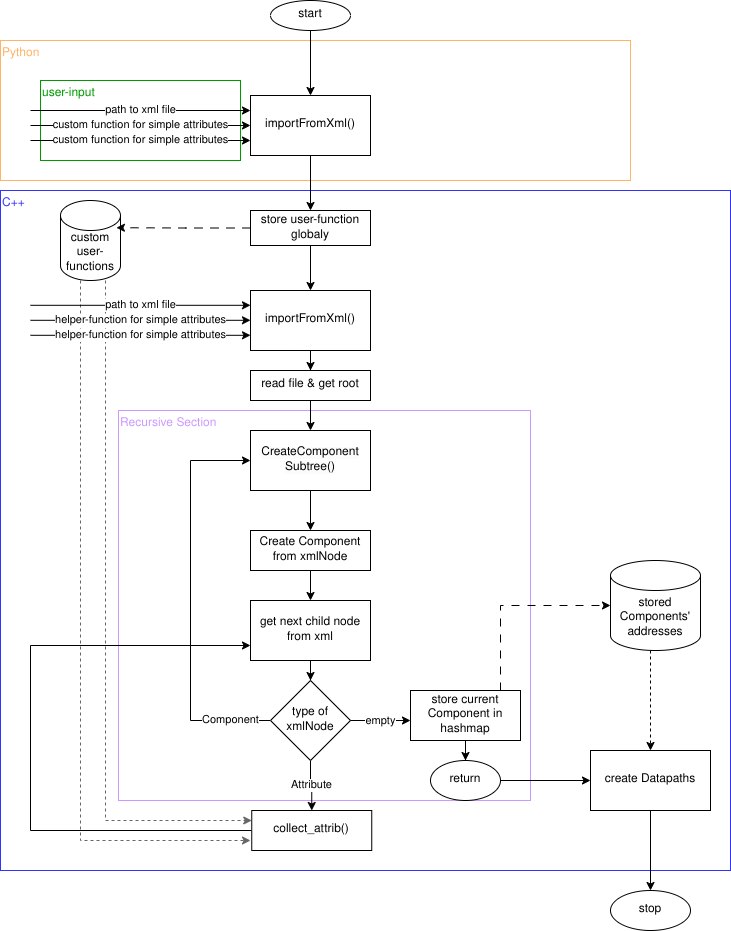
\includegraphics[width=\textwidth]{figures/XML_import-flowchart.png}
    \caption{XML Import Flowchart}
    \label{fig:xml-import}
\end{figure}

\begin{figure}[htpb]
    \centering
    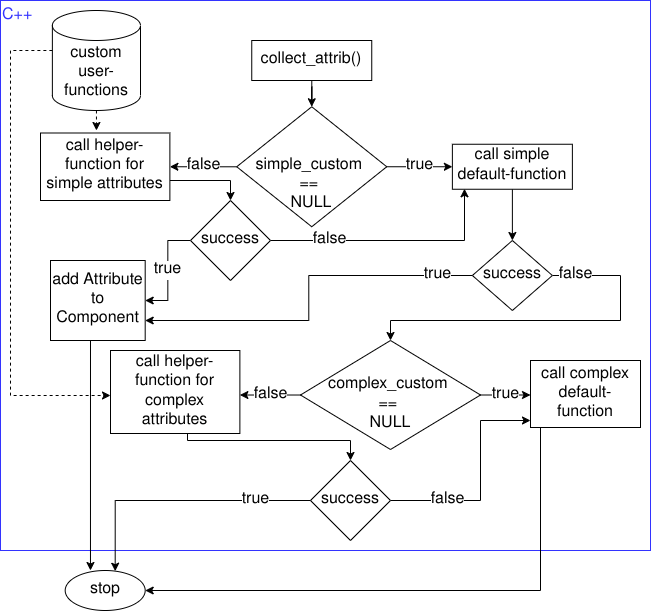
\includegraphics[width=\textwidth]{figures/Attribute_from_xml.png}
    \caption{Attribute parsing}
    \label{fig:Attribute parsing}
\end{figure}
\newpage
\section{Ownership Management and Return-Value Policies}

A critical challenge in interfacing C++ with Python involves the management of object ownership, particularly concerning the \verb|Component| objects within the sys\_sage library. By default, pybind11 transfers ownership of the underlying C++ object to the Python side. This implies that when a Python object, such as \verb|c = sys_sage.Component()|, is created, Python assumes responsibility for its lifecycle, including reference counting and deallocation. While this approach is generally adequate for objects without external dependencies, it becomes problematic when dealing with interconnected components, such as parent-child relationships or datapath associations.

Consider the following scenario:

  \begin{lstlisting}[language=Python, xleftmargin=4em, frame = single]
c = sys_sage.Component()
child = sys_sage.Component(c) # Parent set in constructor
del c
d = child.parent
print(d.id) # Undefined behaviour
  \end{lstlisting}

In this example, deleting \verb|c| in Python leads to the deallocation of the corresponding C++ object. However, the \verb|child| object retains a reference to the now-deleted parent. Consequently, accessing \verb|child.parent| results in undefined behavior, as the referenced object no longer exists. This issue arises because the \verb|Component| destructor does not update references in related objects, such as parent nodes, child nodes, or datapaths.

An initial attempt to address this problem involved implementing a custom delete function, \verb|delete(bool withSubtree)|, to replace the default destructor. However, this approach was deemed unsuitable due to potential conflicts with Python's garbage collection mechanism. As noted in pybind11's documentation, overriding the \verb|__del__(self)| method in Python is strongly discouraged, as it can interfere with the garbage collection process. \cite[see Chapter 12]{python-gc}

To mitigate these issues, pybind11's capability to disable ownership transfer was utilized. By modifying the template parameters of the \verb|py::class_<>| declaration, ownership of the C++ objects can be retained by the C++ side. Specifically, the \verb|std::unique_ptr<Component, py::nodelete>| template parameter was employed. The \verb|py::nodelete| keyword instructs pybind11 to prevent Python from deallocating the underlying C++ object. This ensures that the C++ side remains responsible for managing object lifetimes.

However, this solution introduces a new challenge. The base C++ program provides methods for manually deleting objects, which, when exposed to Python, can lead to inconsistencies. For instance:
\newpage
  \begin{lstlisting}[language=Python, xleftmargin=4em, frame = single]
import sys_sage

c = sys_sage.Component()
d = c
c.Delete()
d.Delete() #Segmentation Fault
  \end{lstlisting}
  

In this scenario, deleting \verb|c| using the \verb|Delete()| method deallocates the C++ object, but the Python wrapper \verb|d| remains unaware of this change. Ideally, all references to the deleted object should be updated. Unfortunately, pybind11 does not provide a mechanism for automatically updating these references. While this scenario is relatively rare, it underscores the need for careful consideration of object deletion strategies.

As mentioned before, pybind11, by default, invokes the destructor of the underlying C++ object when the reference count reaches zero. To enhance consistency, modifying the destructor to update relevant references is considered. 

\subsection{Destructor modifications}

In the base implementation, the destructors remain untouched. Consequently, to free resources, the user must explicitly call the \verb|Delete| function. This function provides the option to also delete the subtree, encompassing all descendants of the component. Naturally, all Datapaths connected to the component are deleted in this process. However, the attributes stored in the \verb|attrib| map are not automatically deallocated. Typically, in most containers from the \ac{STL}, memory is freed upon destruction for all contained items except pointers \cite{cppreference-map-destructor}.

As an alternative to the approach requiring explicit \verb|Delete| calls, thereby passing memory management to the C++ side, we now examine a solution utilizing custom destructors for the Component and Datapath classes. The following illustration, Figure \ref{fig:topo-example}, may help to grasp the details:
\begin{figure}[htpb]
    \centering
    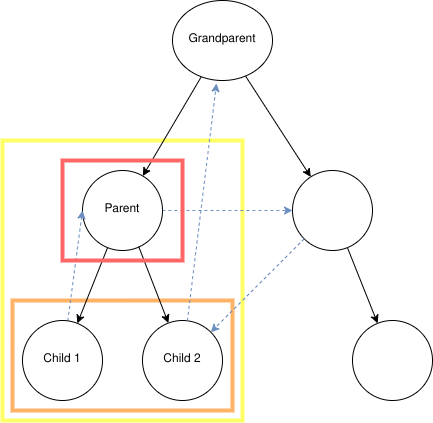
\includegraphics[scale=0.5]{figures/Topo-example.png}
    \caption{Topology Example}
    \label{fig:topo-example}
\end{figure}

To remove the "Parent" in this Topology, we no longer call the \verb|Delete| method. Instead, \verb|delete Parent| is used. In this solution, the Destructor removes all Datapaths connected to the Component. Additionally, Child 1 and 2, as well as the Grandparent, are updated: the children's \verb|parent| values are set to \texttt{NULL}, and Parent is removed from the Grandparent's children list. The children are no longer directly connected to their grandparent and can only be reached if a Datapath to another component remains. In our case, Child 1 becomes unreachable, as its only two connections — once in the Parent's children list and once via the Datapath to Parent — are destroyed with the deletion of Parent. This might also cause memory leaks if components fall out of scope without any remaining connection to the rest of the topology. Therefore, the user should always consider calling the \verb|DeleteSubtree| method beforehand, which has slight modifications compared to the base implementation but effectively achieves the same outcome.

The Datapath's destructor is also modified. Essentially, the logic behind the \verb|DeleteDatapath| method is migrated to the destructor.

The solution presented in this section is cleaner and allows for seamless usage of the pybind11 binding, enabling the Python interpreter to manage memory deallocation.